\documentclass[12pt, a4paper]{article}

\usepackage[utf8]{inputenc}
\usepackage{graphicx}
\graphicspath{ {./images/} }

\title{brief calculator manual}

\author{bgreydon}

\date{March 29 2022}


\begin{document}

% first manual page
\maketitle

\pagebreak

\tableofcontents

\pagebreak

\section{brief introduction}

% main features

% \begin{center}
%   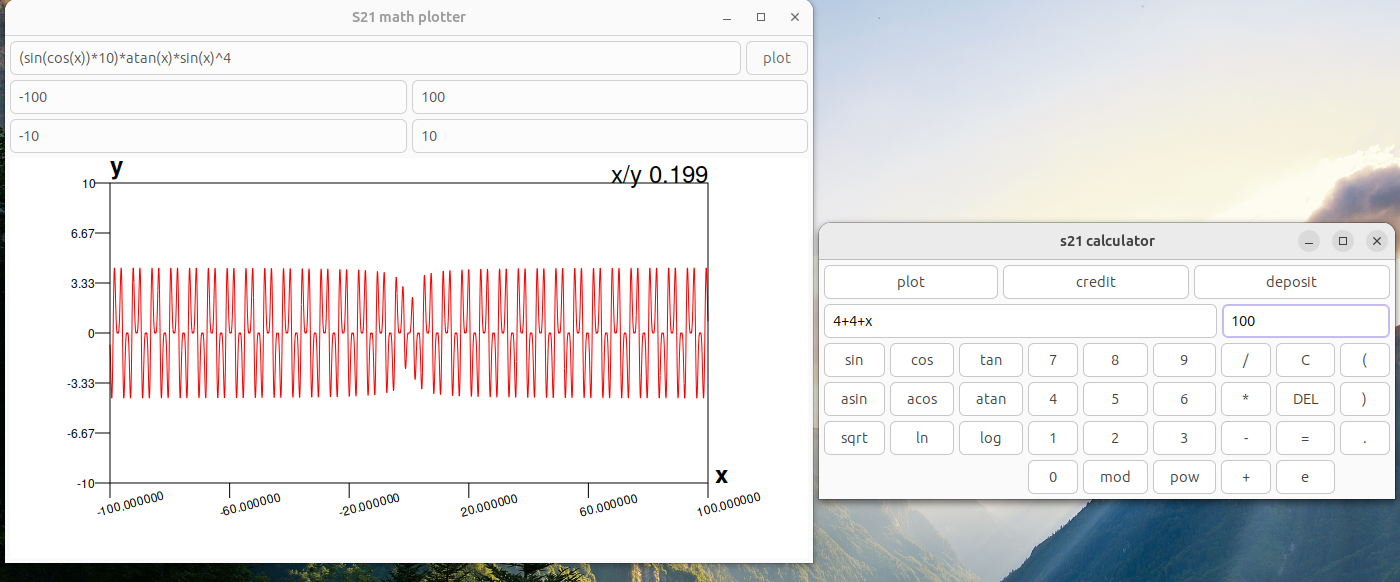
\includegraphics[width=0.8\textwidth]{calc.eps}
% \end{center}

The calculator has a graphical interface written using the gtk 3 library.
Calculator was developed on the Kubuntu 21.10 OS.

The calculators implement mathematical operators, some trigonometric and logarithmic functions. It is possible to set an expression with the variable X and perform a value substitution instead of X. It also has functionality for creating graphs.

At the moment there buttons for calculating \textbf{Deposit} are \textbf{not implemented}.

Calculator can give the answer in exponential form, but does \textbf{not} process expressions in exponential form.

\pagebreak

\section{functions and operators}

The following mathematical operations and functions are implemented in the calculator:
  \begin{itemize}
    \item Arithmetic operators
    \begin{itemize}
      \item Brackets -- "( )"
      \item Addition -- "a + b"
      \item Subtraction -- "a - b"
      \item Multiplication -- "a * b"
      \item Division -- "a / b"
      \item Power -- "a \^\ b"
      \item Modulus -- "a mod b OR a \% b"
      \item Unary plus -- "+a"
      \item Unary minus -- "-a"
    \end{itemize}
    \item Functions
    \begin{itemize}
      \item $cos(x)$
      \item $sin(x)$
      \item $tan(x)$
      \item $acos(x)$
      \item $asin(x)$
      \item $atan(x)$
      \item $sqrt(x)$
      \item $ln(x)$
      \item $log(x)$
    \end{itemize}
  \end{itemize}

\textit{These functions also are supported by the plotter.}

\pagebreak

\section{plotter/grapher}

The grapher/plotter, hereinafter simply the grapher, supports all operators and functions from section 2.

The grapher has the ability to set the domain of definition and the range of value, but it does not have the ability to specify the number of points.

\end{document}
